\documentclass[10pt,a4paper]{article}
\usepackage[utf8]{inputenc}
\usepackage[spanish,es-nodecimaldot]{babel}
\usepackage{amsmath,amssymb,geometry,hyperref,fancyhdr,microtype,booktabs,graphicx}
\graphicspath{{../resultados/}{./}}
\geometry{margin=2cm}
\pagestyle{fancy}\fancyhf{}
\fancyhead[L]{\small Universidad Externado de Colombia}
\fancyhead[R]{\small Métodos Numéricos -- Proyecto Integrador (Entrega Final)}
\fancyfoot[C]{\thepage}
\hypersetup{colorlinks=true,linkcolor=black,citecolor=black,urlcolor=blue}

\begin{document}
\begin{titlepage}\centering\vspace*{2cm}
{\LARGE\bfseries Proyecto Integrador: Entrega Final}\\[.5cm]
{\large Implementación reproducible, estabilidad dinámica y análisis para raíces múltiples}\\[.6cm]
{\Large Métodos Numéricos}\\[2cm]
Integrantes: Ailyn Sofía Gómez Rodríguez, Julián Camilo Jiménez Rodríguez, Julián Steven Duarte\\[1cm]
Docente: Edwin Fernando Muñoz Chipatecua\vfill 
Pregrado en Ciencia de Datos\\
Departamento de Matemáticas\\
Universidad Externado de Colombia\\
Bogotá D.C., Colombia -- Noviembre de 2026
\end{titlepage}

\section{Planteamiento del problema y objetivo}
En ecuaciones no lineales $g(x)=0$ con raíces de multiplicidad conocida $m > 1$, la anulación de las primeras $m-1$ derivadas ($g'(x)\to 0$) degrada la convergencia cuadrática del método de Newton clásico a orden estrictamente lineal ($p=1$), amplificando la cancelación numérica \cite{turner}. El método de Newton modificado ($x_{k+1}=x_k - m g(x_k)/g'(x_k)$) recupera el orden cuadrático ($p=2$), pero requiere el cálculo explícito de $g'(x)$, computacionalmente costoso o inviable en aplicaciones de ciencia de datos.

Jerezano, Chicharro y Garrido-Sáez (2026) propusieron una familia de métodos iterativos libre de derivadas de orden cuatro que aprovecha el conocimiento de $m$ \cite{jerezano}. El objetivo de esta entrega final es consolidar la implementación de sus dos variantes principales, evaluar experimentalmente su estabilidad en el plano complejo, contrastar rigurosamente los resultados numéricos frente a las tablas del artículo base, explorar una extensión a sistemas no lineales y discutir su relevancia en optimización y ciencia de datos.

\section{Métodos numéricos y optimalidad de Kung-Traub}
Dada la pendiente secante $g[w_k,x_k]=(g(w_k)-g(x_k))/(w_k-x_k)$, el esquema multipaso de Jerezano et al. define:
\begin{align*}
w_k&=x_k+\beta g(x_k)^2,\quad (\beta\neq 0), & y_k&=x_k-m\frac{g(x_k)}{g[w_k,x_k]},\\
t_k&=\left(\frac{g(y_k)}{g(x_k)}\right)^{1/m}, & x_{k+1}&=x_k-mH(t_k)\frac{g(x_k)}{g[w_k,x_k]}.
\end{align*}
Para evaluar potencias fraccionarias con base real negativa en etapas transitorias, se emplea la rama principal del logaritmo complejo: $t_k=\exp\left(\frac{1}{m}\operatorname{Log}\left(\frac{g(y_k)}{g(x_k)}\right)\right)$, con argumento $\operatorname{Arg}(z)\in(-\pi,\pi]$. Esta elección aporta una convención unívoca para el cómputo, asumiendo la discontinuidad del corte de rama sobre el semieje real negativo.

\textbf{Optimalidad teórica de Kung-Traub.} La conjetura de Kung y Traub (1974) establece que un método multipaso sin memoria con $d$ evaluaciones funcionales por ciclo alcanza un orden de convergencia máximo de $p\le 2^{d-1}$ \cite{kungtraub}. Al evaluar únicamente tres valores de función ($g(x_k), g(w_k), g(y_k)$) y ninguna derivada ($d=3$), el orden óptimo es $p=4$. De acuerdo con el Teorema 2 del artículo, dicho orden se obtiene si la función de peso satisface $H(0)=1$, $H'(0)=1$, $H''(0)=4$ y $|H'''(0)|<\infty$. Las dos variantes analizadas satisfacen plenamente estas condiciones:
\begin{itemize}
\item \textbf{M1 (ponderación polinomial cuadrática):} $H_1(t)=1+t+2t^2$, donde $H_1'''(0)=0<\infty$.
\item \textbf{M2 (ponderación racional):} $H_2(t)=\frac{1-t}{1-2t}$, con $H_2'''(0)=24<\infty$ y polo en $t=1/2$.
\end{itemize}
Ambas variantes alcanzan un índice de eficiencia computacional teórico $\mathcal{I}=4^{1/3}\approx 1.587$, superior a $\mathcal{I}=2^{1/2}\approx 1.414$ de Newton modificado y Steffensen modificado ($w_k=x_k+\beta g(x_k)$). Como medida teórica, este índice no implica necesariamente un menor tiempo de cómputo en CPU. Para benchmarking se incluye también el método de Kumar et al. (KK, 2020) \cite{kk}, de orden cuatro libre de derivadas.

\section{Estabilidad y dinámica en el plano complejo}
Sobre el polinomio canónico cuadrático $p(z)=(z-1)^2$ ($m=2$), el esquema genera un operador racional de punto fijo $z_{k+1}=R(z,\beta)$. La raíz $z^*=1$ es un \textbf{punto fijo superatractor} ($R'(1,\beta)=0$), garantizando convergencia local de orden superior en una vecindad de la raíz.

\begin{figure}[htbp]
\centering
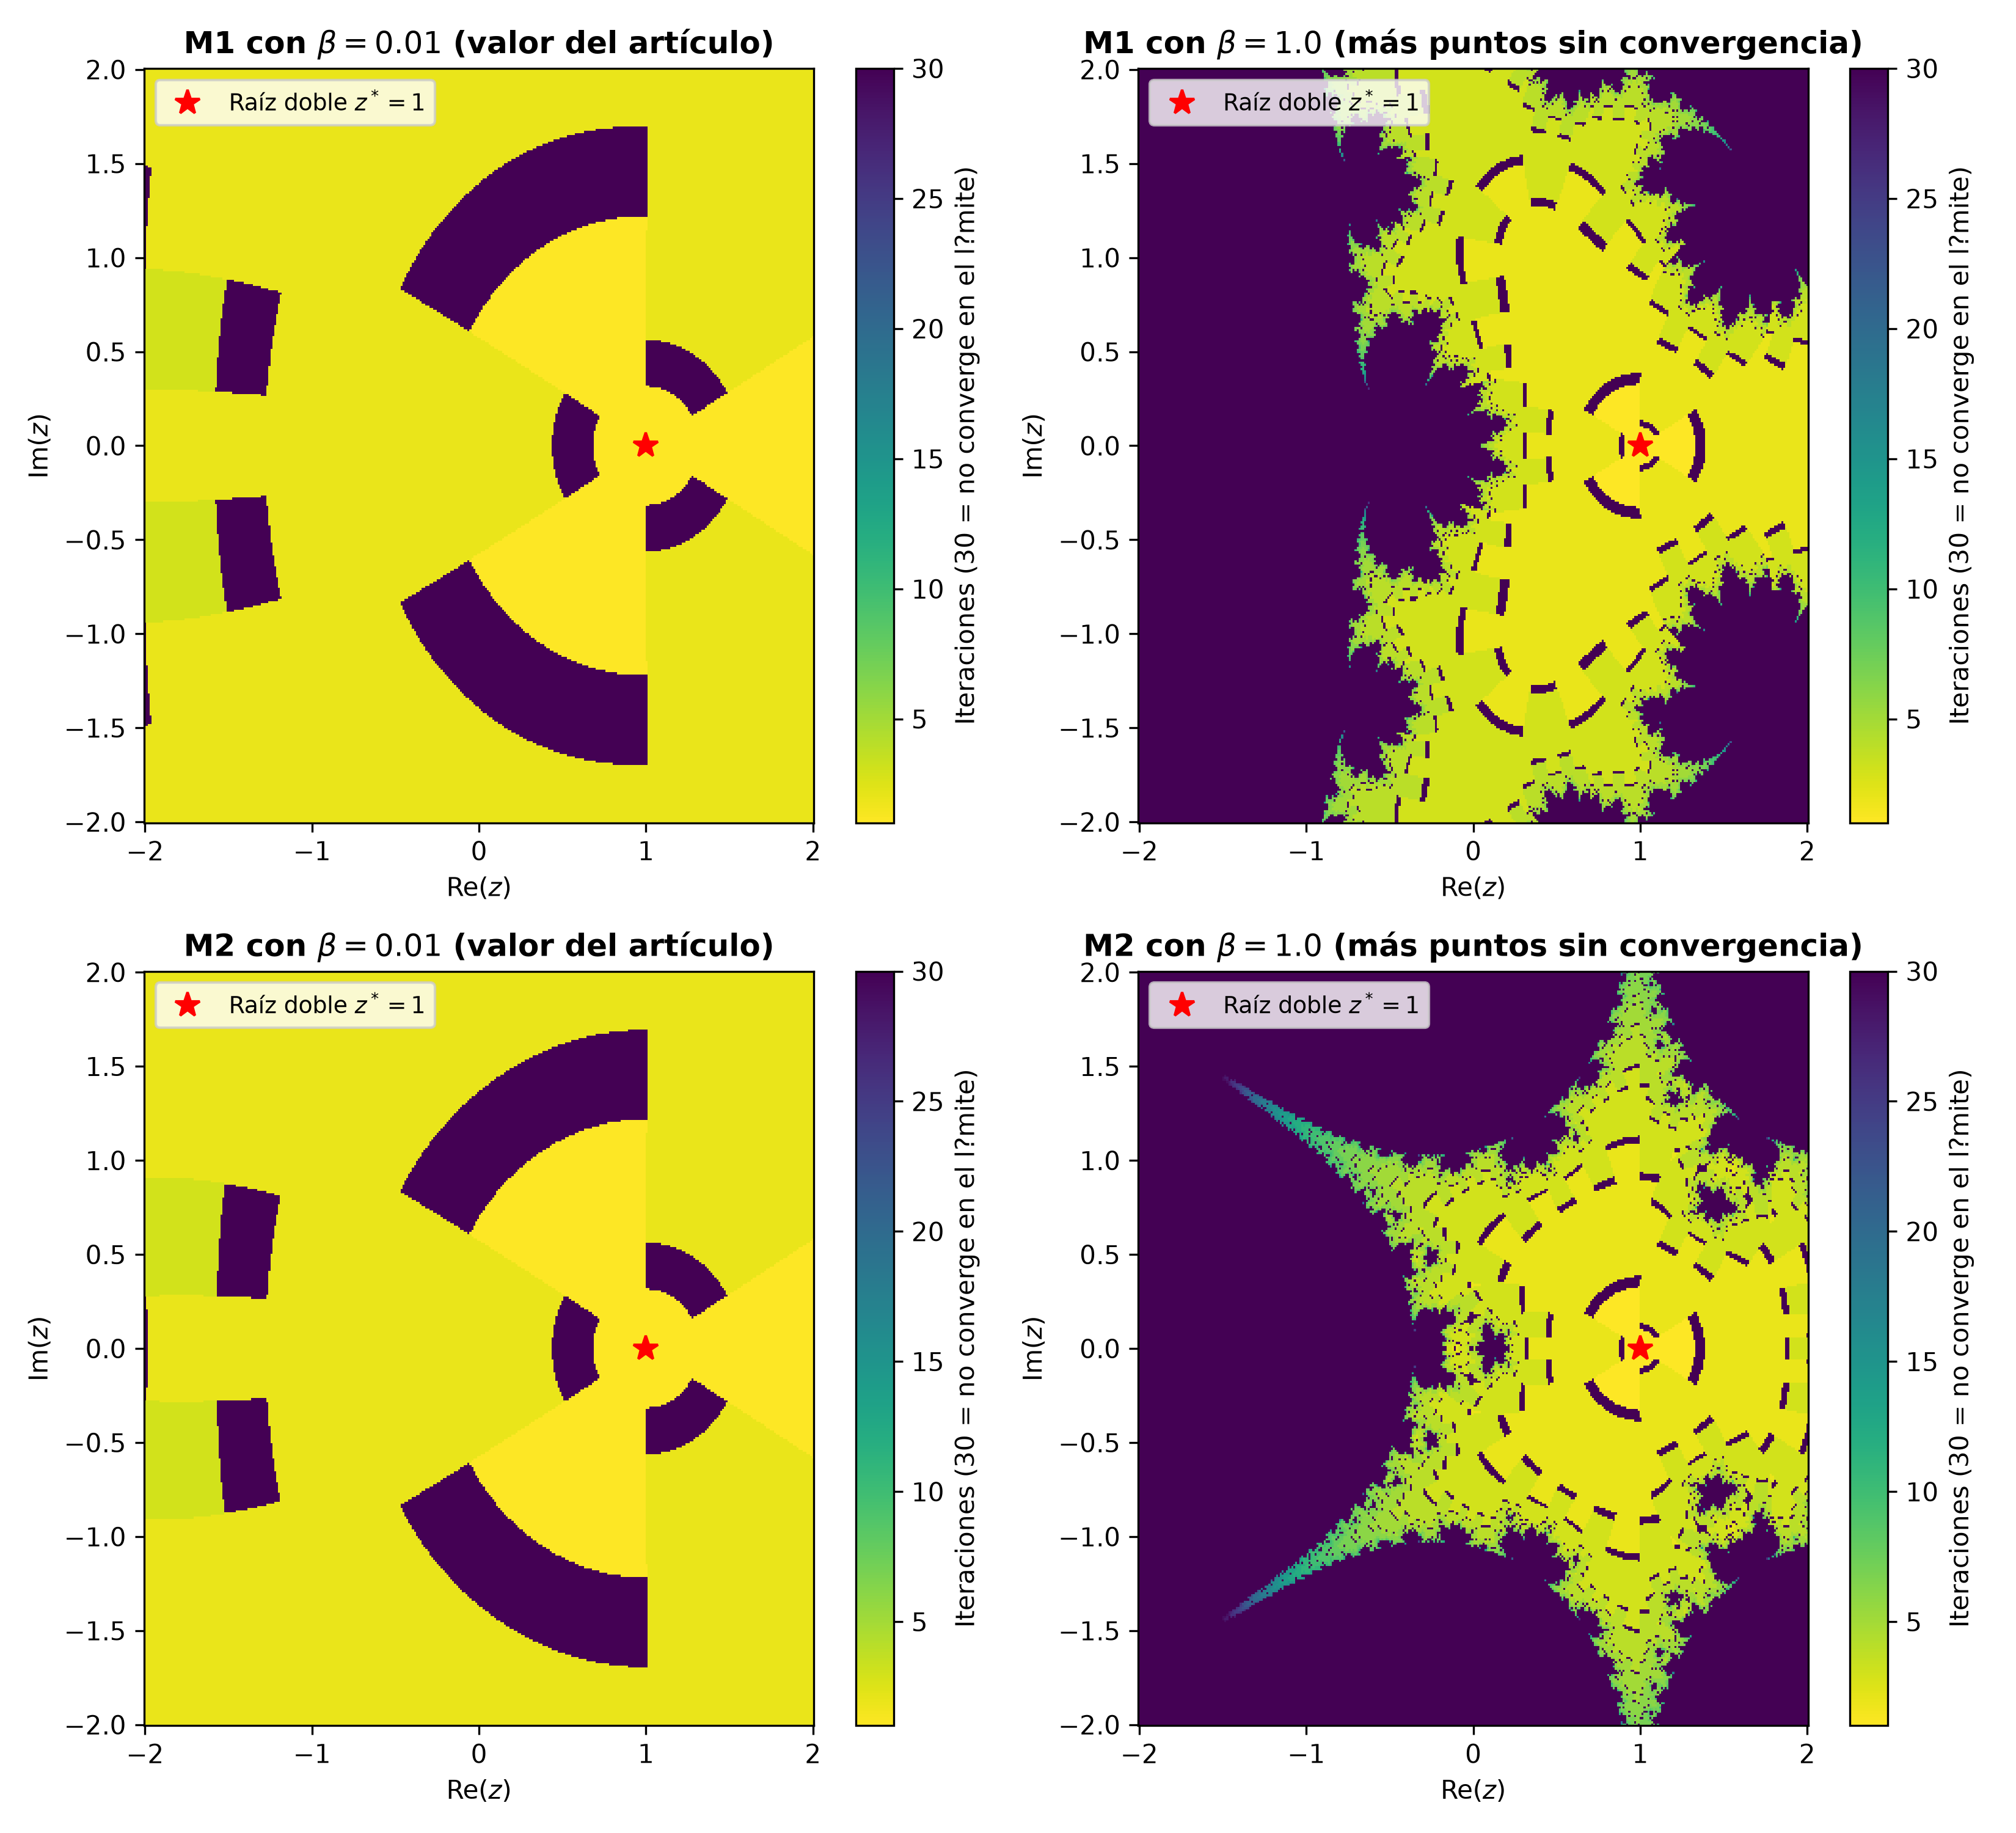
\includegraphics[width=0.78\textwidth]{dinamica_compleja_m1_m2.png}
\caption{Planos dinámicos en $[-2,2]\times[-2,2]$ (malla $350\times 350$, máx. 30 iteraciones) para M1 y M2 con $\beta\in\{0.01, 1.0\}$. Los puntos en 30 indican no convergencia en el límite fijado.}
\label{fig:dinamica}
\end{figure}

La Figura~\ref{fig:dinamica} ilustra la convergencia en una malla uniforme de $350\times 350$ puntos en $[-2,2]\times[-2,2]$ (ajuste computacional frente a la malla de $1000\times 1000$ en $[-20,20]\times[-20,20]$ del artículo). Se confirma que con $\beta=0.01$ la cuenca de convergencia efectiva es amplia y regular, mientras que $\beta=1.0$ incrementa las zonas de terminación tardía. Este ensayo delimita cuencas numéricas finitas sin constituir una caracterización matemática exhaustiva de conjuntos de Fatou y Julia.

\section{Problemas de prueba y diseño experimental}
Se evaluaron los problemas deterministas del artículo base, sin muestreo aleatorio:
\begin{enumerate}
\item \textbf{$g_1(x)=x^3-5.22x^2+9.0825x-5.2675$:} Modelo de Van der Waals con raíz doble en $\alpha_1=1.75$ ($m=2$) y raíz simple en $\alpha_2=1.72$. Semillas: $x_0\in\{1.9, 3.0\}$.
\item \textbf{$g_2(x)=(e^{-x}-1+x/5)^3$:} Ecuación de radiación de Planck al cubo. Posee dos raíces de multiplicidad tres: $x=0$ y la raíz positiva de estudio $\alpha\approx 4.96511423$ ($m=3$). Semillas: $x_0\in\{5.3, 10.0\}$.
\item \textbf{$g_3(x)=x^9-29x^8+349x^7-2261x^6+8455x^5-17663x^4+15927x^3+6993x^2-24732x+12960$:} Polinomio característico con raíz cuádruple en $\alpha=3$ ($m=4$). Semillas: $x_0\in\{2.8, 3.4, 3.5\}$.
\end{enumerate}

\section{Configuración computacional, precisión y parada}
El entorno experimental en Python utiliza \texttt{mpmath} con precisión de 150 dígitos decimales (\texttt{dps=150}), cota máxima de 100 iteraciones y parámetro base $\beta=0.01$.

\textbf{Criterio dual estricto y resolución finita.} En raíces múltiples, el residuo decae como $|x-\alpha|^m$. Por ejemplo, en $g_3(x)\approx -80(x-3)^4$, un residuo de $10^{-68}$ se produce con un error de apenas $10^{-18}$. Para evitar falsas paradas prematuras, el algoritmo exige simultáneamente:
\[ |\Delta x_k| = |x_{k+1}-x_k| < 10^{-25} \quad \text{y} \quad |g(x_{k+1})| < 10^{-25}. \]
Si la perturbación $\beta g(x_k)^2$ resulta demasiado pequeña para modificar la representación numérica de $x_k$ bajo la precisión configurada, el código detecta la igualdad computacional $w_k=x_k$ y detiene la ejecución por \texttt{Estancamiento w=x}, evitando divisiones por cero indeterminadas. Asimismo, se capturan singularidades por derivadas o pendientes nulas.

\textbf{Orden computacional (ACOC).} Se estima el orden local mediante el índice de Cordero-Torregrosa (2007) \cite{cordero}, empleando tres diferencias consecutivas de paso:
\[ \mathrm{ACOC}\approx \frac{\ln(|\Delta x_{k+1}|/|\Delta x_k|)}{\ln(|\Delta x_k|/|\Delta x_{k-1}|)}. \]
Su cálculo se restringe a métodos convergentes con al menos cuatro iterados en régimen asintótico terminal.

\section{Resultados experimentales y análisis comparativo}
El Cuadro~\ref{tab:resultados_finales} resume el desempeño comparativo en CPU Intel Core i5-12500H (promedio de 10 ejecuciones deterministas consecutivas). El detalle completo de todas las combinaciones y casos no convergentes se conserva en el cuaderno adjunto y en \texttt{resultados\_fase3.csv}.

\begin{table}[htbp]
\centering
\caption{Resultados comparativos representativos (150 dígitos, $\mathrm{TOL}=10^{-25}$, $\beta=0.01$).}
\label{tab:resultados_finales}
\small
\resizebox{\textwidth}{!}{
\begin{tabular}{llrrrrrrrrl}
\toprule
Problema & Método & Iter. & $g$ eval. & $g'$ eval. & Error abs. & $|\Delta x_k|$ & Residuo & ACOC & $T$ (ms) & Estado \\
\midrule
$g_1$, $x_0=1.9$ & M1 & 5 & 17 & 0 & $1.32\times10^{-35}$ & $9.51\times10^{-66}$ & $5.26\times10^{-72}$ & 8.81 & 1.7 & Convergió \\
$g_1$, $x_0=1.9$ & M2 & 4 & 14 & 0 & $2.03\times10^{-50}$ & $4.14\times10^{-14}$ & $1.24\times10^{-101}$ & -- & 1.3 & Estancamiento $w=x$ \\
$g_1$, $x_0=1.9$ & Newton mod. & 8 & 10 & 8 & $1.69\times10^{-57}$ & $1.01\times10^{-29}$ & $8.58\times10^{-116}$ & 2.00 & 1.1 & Convergió \\
$g_1$, $x_0=1.9$ & Steffensen & 8 & 18 & 0 & $1.77\times10^{-57}$ & $1.03\times10^{-29}$ & $9.43\times10^{-116}$ & 2.00 & 1.4 & Convergió \\
$g_1$, $x_0=1.9$ & KK & 4 & 15 & 0 & $1.01\times10^{-53}$ & $6.83\times10^{-15}$ & $3.06\times10^{-108}$ & -- & 1.5 & Pendiente secante nula \\
\midrule
$g_1$, $x_0=3.0$ & Newton mod. & 10 & 12 & 10 & $2.61\times10^{-62}$ & $3.96\times10^{-32}$ & $2.05\times10^{-125}$ & 2.00 & 1.2 & Convergió \\
$g_1$, $x_0=3.0$ & Steffensen & 10 & 22 & 0 & $5.52\times10^{-61}$ & $1.82\times10^{-31}$ & $9.14\times10^{-123}$ & 2.00 & 1.6 & Convergió \\
$g_1$, $x_0=3.0$ & KK & 6 & 20 & 0 & $1.63\times10^{-55}$ & $1.04\times10^{-74}$ & $7.95\times10^{-112}$ & 5.91 & 2.1 & Convergió \\
\midrule
$g_2$, $x_0=5.3$ & M1 & 2 & 8 & 0 & $2.07\times10^{-28}$ & $1.11\times10^{-6}$ & $6.41\times10^{-86}$ & -- & 0.7 & Estancamiento $w=x$ \\
$g_2$, $x_0=5.3$ & Newton mod. & 5 & 7 & 5 & $1.45\times10^{-71}$ & $2.83\times10^{-35}$ & $2.18\times10^{-215}$ & 2.00 & 0.9 & Convergió \\
$g_2$, $x_0=5.3$ & KK & 3 & 11 & 0 & $9.91\times10^{-117}$ & $9.65\times10^{-29}$ & $7.01\times10^{-351}$ & 3.97 & 1.1 & Convergió \\
\midrule
$g_3$, $x_0=2.8$ & M1 & 3 & 11 & 0 & $3.71\times10^{-18}$ & $5.62\times10^{-60}$ & $1.52\times10^{-68}$ & -- & 1.6 & Criterio dual; error $>$ TOL \\
$g_3$, $x_0=2.8$ & M2 & 3 & 11 & 0 & $5.42\times10^{-19}$ & $4.19\times10^{-123}$ & $6.89\times10^{-72}$ & -- & 1.6 & Criterio dual; error $>$ TOL \\
$g_3$, $x_0=3.4$ & M1 & 4 & 14 & 0 & $2.16\times10^{-17}$ & $3.72\times10^{-51}$ & $1.75\times10^{-65}$ & -- & 1.9 & Criterio dual; error $>$ TOL \\
$g_3$, $x_0=3.4$ & M2 & 4 & 14 & 0 & $3.90\times10^{-17}$ & $5.27\times10^{-80}$ & $1.84\times10^{-64}$ & -- & 1.9 & Criterio dual; error $>$ TOL \\
$g_3$, $x_0=3.5$ & M1 & 100 & 301 & 0 & $1.04$ & $7.30\times10^{-15}$ & $1.23\times10^{2}$ & -- & 95.1 & Límite de iteraciones \\
\bottomrule
\end{tabular}}
\end{table}

\begin{figure}[htbp]
\centering
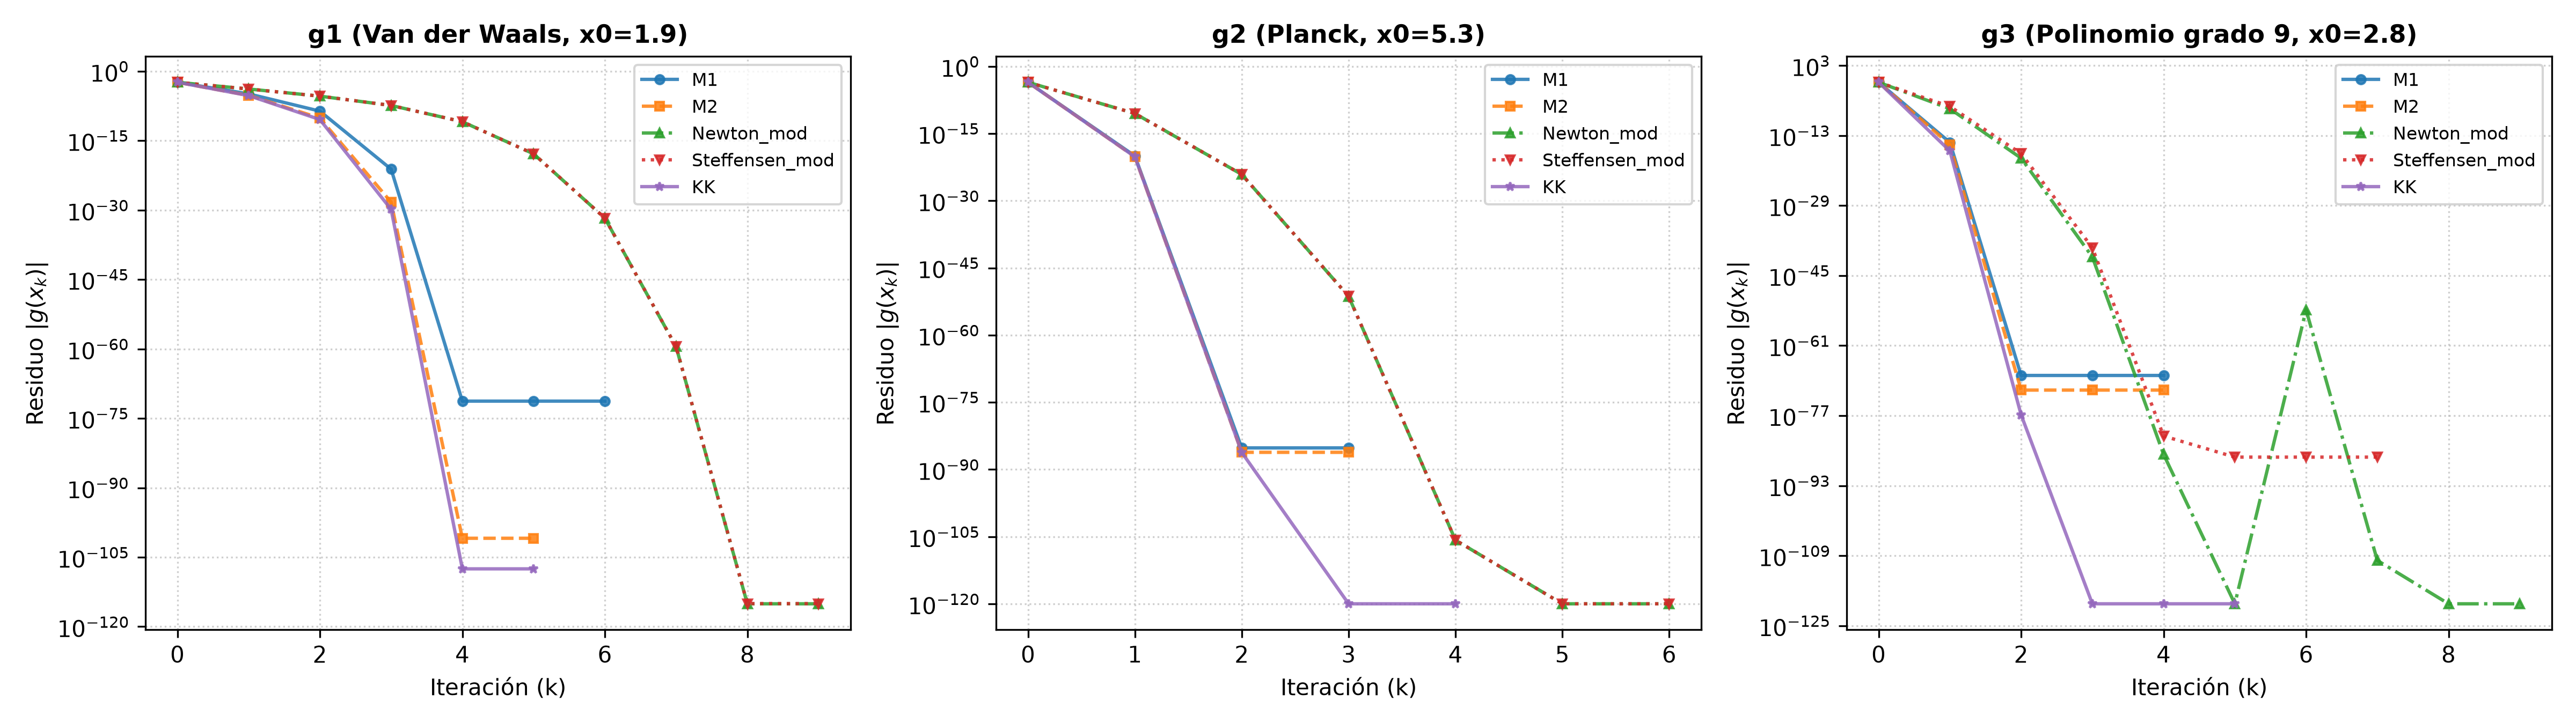
\includegraphics[width=0.86\textwidth]{convergencia_residuos.png}
\caption{Perfiles de convergencia del residuo $|g(x_k)|$ en escala logarítmica.}
\label{fig:convergencia}
\end{figure}

\textbf{Interpretación técnica de los resultados:}
\begin{itemize}
\item \textbf{Conteo transparente de evaluaciones:} En M1 y M2, cada paso evalúa $g(x_k)$, $g(w_k)$ y $g(y_k)$. El solucionador añade $g(x_0)$ inicial y una llamada post-bucle $g(x_{\mathrm{final}})$ para registro independiente, totalizando $1+3k+1$ evaluaciones ($17$ para $k=5$). En métodos abortados, se auditan únicamente las llamadas efectivamente completadas (p.~ej., 15 evaluaciones en KK antes de fallar el denominador).
\item \textbf{Estancamiento controlado:} En $g_1$ ($x_0=1.9$, M2), tras 4 pasos ($|\Delta x_4|\approx 4.14\times 10^{-14}>\mathrm{TOL}$), la perturbación $\beta g(x_4)^2\approx 1.5\times 10^{-204}$ no altera la mantisa de 150 dígitos de $x_4$. La igualdad $w_5=x_4$ fuerza la parada preventiva por absorción numérica, a pesar de que la aproximación presenta un error absoluto muy pequeño ($10^{-50}$).
\item \textbf{Terminación operativa frente a exactitud efectiva en $g_3$ ($m=4$):} Para $x_0=2.8$, los pasos finales colapsan ($|\Delta x_3|<10^{-59}$) y los residuos son menores a $10^{-67}$, satisfaciendo formalmente la tolerancia dual en 3 iteraciones. No obstante, los errores absolutos frente a la raíz exacta $\alpha=3$ son de orden $10^{-18}$ y $10^{-19}$. Esta dinámica evidencia que en multiplicidades altas, la convergencia del residuo antecede con creces a la cercanía real a la raíz, por lo que el estado se clasifica honestamente como \texttt{Criterio dual; error > TOL}.
\end{itemize}

\textbf{Contraste frente al artículo base:}
\begin{itemize}
\item \textbf{Coincidencias:} La familia M1/M2 reduce el residuo de forma marcadamente más acelerada por ciclo que Newton modificado sin requerir derivadas analíticas (Figura~\ref{fig:convergencia}).
\item \textbf{Diferencias y causas técnicas:} Para $g_1$ ($x_0=1.9$), el artículo reporta 7 iteraciones frente a 5 en nuestra corrida. Para $g_3$ ($x_0=2.8$), los autores reportan 5 iteraciones mientras nuestra implementación satisface el criterio dual en 3 pasos; sin embargo, al presentar errores absolutos superiores a la tolerancia, esta diferencia no indica superioridad algorítmica sino una terminación anticipada propiciada por las condiciones de parada ($10^{-25}$ con 150 dígitos frente a $10^{-200}$ con 4000 dígitos en el artículo).
\end{itemize}

\section{Experimento complementario: extensión multidimensional}
Para ilustrar la relevancia de los esquemas sin derivadas en varias dimensiones (Semana 9 del curso \cite{turner}), se resolvió el sistema no lineal:
\[ \mathbf{F}(x_1, x_2) = \begin{pmatrix} x_1^2 + x_2^2 - 4 \\ x_1 x_2 - 1 \end{pmatrix} = \mathbf{0}, \quad \text{con } \mathbf{x}_0 = (1.5, 0.8)^T. \]
Newton multivariable convergió a la raíz $\mathbf{x}^*\approx (1.93185, 0.51764)^T$ en 5 iteraciones con residuo $3.92\times 10^{-15}$, requiriendo evaluar 20 derivadas parciales y resolver 5 sistemas lineales. El método secante de Broyden alcanzó la misma precisión en 10 iteraciones sin calcular derivadas analíticas, mediante actualizaciones de rango uno de la aproximación Jacobiana. Este ensayo ilustra el compromiso entre número de iteraciones y costo por evaluación que inspira el desarrollo de métodos libres de derivadas en problemas multidimensionales.

\section{Alcance en ciencia de datos, optimización y conclusiones}
En aprendizaje automático, el entrenamiento de modelos busca puntos críticos $\nabla L(\boldsymbol{\theta})=\mathbf{0}$. En paisajes de pérdida mal condicionados (puntos de ensilladura o mesetas degeneradas), la matriz Hessiana posee autovalores cercanos a cero, asemejándose a multiplicidades analíticas donde los métodos estándar se ralentizan.

\textbf{Conclusiones y trabajo futuro:} La familia de Jerezano et al. valida experimentalmente las ventajas del orden cuatro libre de derivadas, alcanzando optimalidad teórica. Sin embargo, su desempeño práctico depende fuertemente de la precisión aritmética disponible para evitar el estancamiento por absorción de la perturbación $\beta g(x_k)^2$. La principal limitación radica en asumir conocida la multiplicidad exacta $m$. Como trabajo futuro se propone la estimación adaptativa de $m$ durante las etapas iniciales y su generalización a problemas de optimización estocástica.

\textbf{Integridad académica:} Se utilizó asistencia de herramientas de IA para revisión editorial y estructuración del código conforme a las directrices de la guía del proyecto \cite{guia}. El equipo comprende y sustenta plenamente todos los fundamentos matemáticos y resultados reportados.

\begin{thebibliography}{9}\small
\bibitem{cordero} A. Cordero y J. R. Torregrosa, ``Variants of Newton's method using fifth-order quadrature formulas'', \emph{Appl. Math. Comput.}, vol. 190, no. 1, pp. 686--698, 2007.
\bibitem{jerezano} J. H. Jerezano, F. I. Chicharro y N. Garrido-Sáez, ``Derivative-free optimal multiple-root finding family of iterative methods'', \emph{Comput. Appl. Math.}, vol. 45, art. 304, 2026.
\bibitem{kungtraub} H. T. Kung y J. F. Traub, ``Optimal order of one-point and multipoint iteration'', \emph{J. ACM}, vol. 21, no. 4, pp. 643--651, 1974.
\bibitem{kk} S. Kumar et al., ``An optimal fourth order derivative-free numerical algorithm for multiple roots'', \emph{Symmetry}, vol. 12, no. 6, art. 1038, 2020.
\bibitem{turner} P. R. Turner, T. Arildsen y K. Kavanagh, \emph{Applied Scientific Computing: With Python}, Springer, Cham, 2018.
\bibitem{guia} Universidad Externado de Colombia, \emph{Guía del Proyecto Integrador: Métodos Numéricos}, 2026.
\end{thebibliography}

\end{document}
